\documentclass[6pt]{article}
\usepackage[paperwidth=5.5in, paperheight=4.25in, top=0.25in, left=0.25in, right=0.75in, bottom=0.25in]{geometry}
\usepackage{graphicx}

\usepackage[light]{antpolt}
\usepackage[T1]{fontenc}
\usepackage[gen]{eurosym}


\usepackage[none]{hyphenat}

\usepackage[utf8]{inputenc}

\begin{document}
\pagestyle{empty}

\centering{
  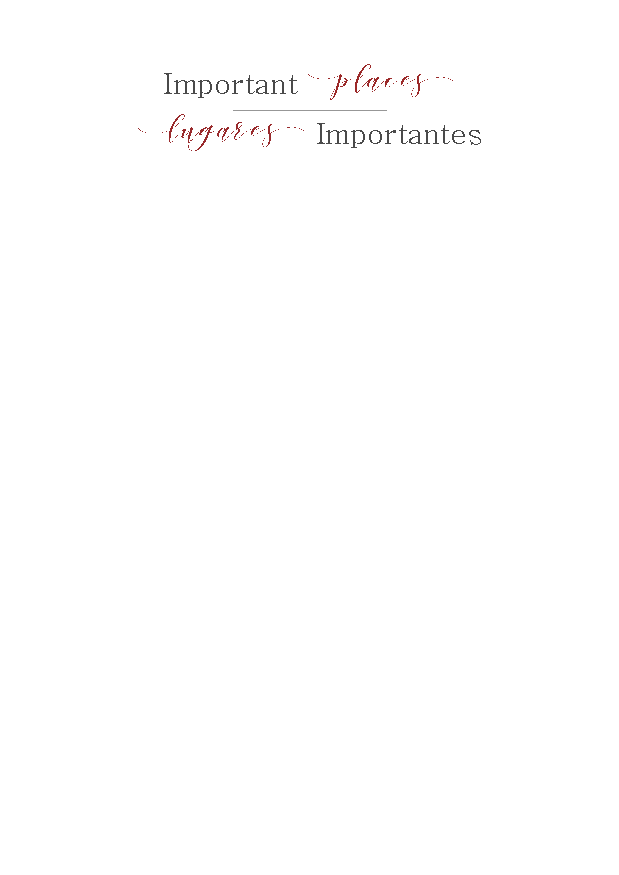
\includegraphics[height=0.75in]{img/important_places}\\
}
\small
{\bf Where is the Quinta dos Machados?} / 
{\bf Onde fica a Quinta dos Machados?} \\


Quinta dos Machados\\
E.N. 8 Barras\\
2665-006 Mafra\\

\vspace{10pt}

{\bf Where is the church?} / {\bf Onde fica a igreja?}\\
Igreja São Silvestre\\
Rua das Forças Armadas\\
2665-118 Gradil

\vspace{10pt}

\begin{tabular}{p{2.125in}|p{2.125in}}

{\bf How may I reserve a room at the hotel?}
&
{\bf Como posso reservar o quarto no hotel?}
\\
To reserve your room, you can call +351 261-96-12-79 or email quintamachados@quintamachados.com. You should mention the secret code for the wedding: Justine.Ruben.20.05. Rooms range from 80\euro{}-115\euro{}/night.
&
Para reservar o seu quarto, telefonar para +351 261 96 12 79 ou enviar um email para quintamachados@quintamachados.com. Deve mencionar o código secreto: Justine.Ruben.20.05. O preço dos quartos varia entre 80\euro{}-115\euro{}/noite.\\
\end{tabular}
\end{document}
